% ==================================================
% CHAPTER 3: Using cosmic muon data for alignment studies
% ==================================================

\chapter{Using cosmic muon data for alignment studies}

The cosmic muon data collected is high in statistics, and the clean trail of ionization left by the muons leaves a clean signal.

% --------------------------------------------------
\section{Measuring alignment using cosmics data}
% --------------------------------------------------

Misalignments can be modeled as passive transformations. Ideally, a misalignment model would be chosen and the parameters (for example, a global offset and rotation for each layer) calculated. To understand the potential of cosmic muon data, it is useful to define a local offset. For each area of a strip layer, the local offset is the offset of the strip pattern in that area with respect to the nominal geometry.  Local offsets systematically change the strip that is hit by a muon passing through the area. The \package{tgc\_analysis/CosmicsAnalysis} software assumes the nominal geometry, so the recorded muon y-position ($y_{cluster}$) is shifted opposite to the local offset ($d_{local}$),
% Maybe useful sentence?: The local offset is a result of the non-conformities in the strip pattern etching and inter-layer misalignments.
\begin{equation}
    y_{cluster} = y_{nom} - d_{local}
    \label{eqn:local_translation}
\end{equation}
% Maybe useful sentence?: The true position of individual cosmic muons is not known, and in the analysis the four detector planes float with respect to a software-implemented origin that is not associated with a fixed physical location.
where $y_{nom}$ is the position of the muon that would have been recorded if there was no local offset. Equation~\ref{eqn:local_translation} ignores other factors that could affect the cluster position (like resolution). The local offset is unknown and there is no external reference to measure $y_{nom}$. Therefore, only relative alignment parameters can be extracted. The minimal relative coordinate system uses two reference or fixed layers~\cite{lefebvre_thesis}. The hits on the two fixed layers are used to create a track that can be interpolated or extrapolated to the other two layers. The residual of track $i$, $\Delta_i$ is defined as,
\begin{equation}
    \Delta_i = y_{i,hit} - y_{i,track}
    \label{eqn:residual}
\end{equation}

Track residuals are affected by the local offset in the area of each layer's hit. As an example, in figure~\ref{fig:fake_event_display}, layers 1 and 4 are used as reference, and the residual on layer 2 perhaps indicates that in the area of the track, layer 3 is offset with respect to layers 1 and 4. However, there is no way to parse out if is it really layer 2 that is offset with respect to the nominal geometry, or some combination of offset on all three layers that causes the residual.

\begin{figure}
    \centering
    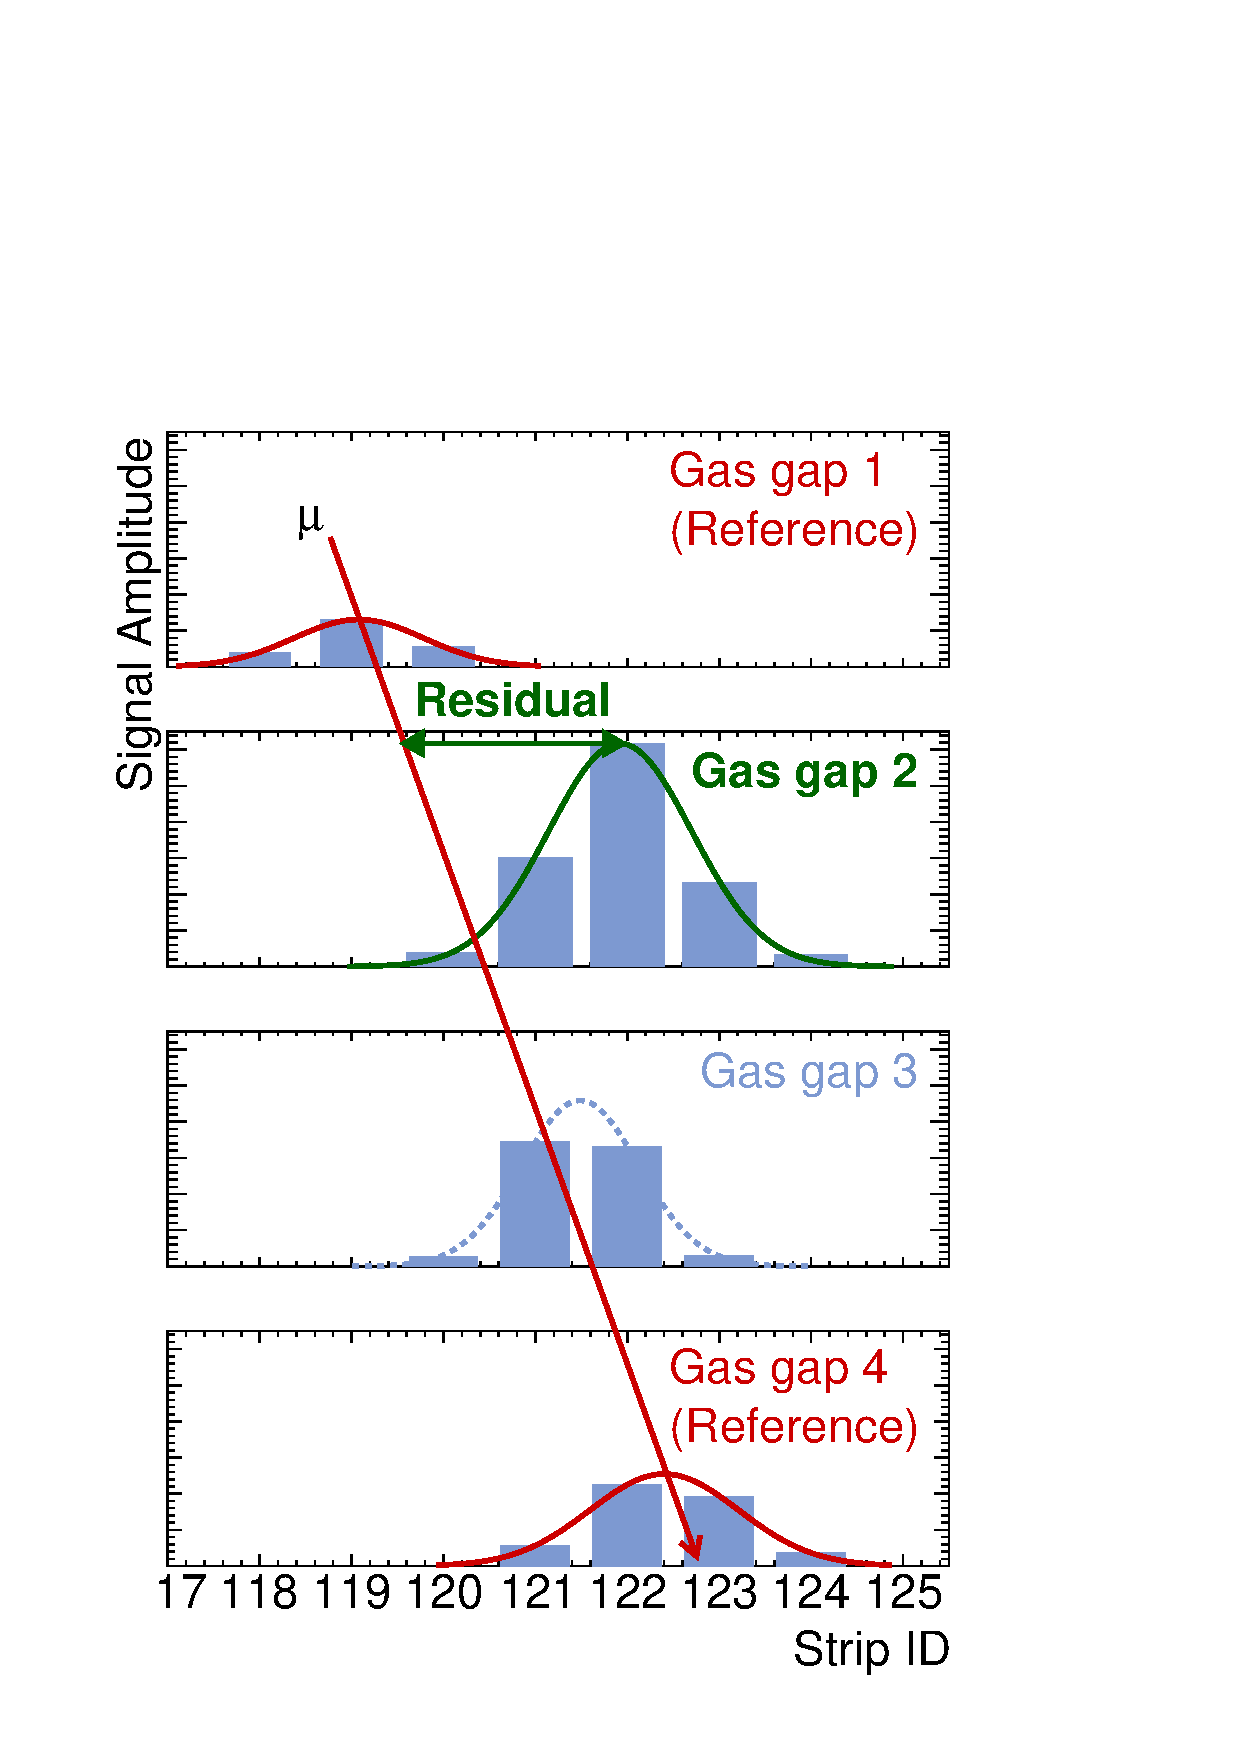
\includegraphics[width = 0.95\textwidth]{figures/figure_fake_event_display.pdf}
    \caption{Representation of a muon event recorded by an sTGC. The clusters are fit with a Gaussian and the mean is taken as the hit position. A track is built from the chosen reference layers, 1 and 4, and the residual calculated on layer 2.}
    \label{fig:fake_event_display}
\end{figure}

Of course, a single track residual says nothing of the real relative local offset because of the limited spatial resolution of the detectors and tracks caused by noise or delta rays contributing large residuals. However, the mean of residuals for all tracks in a region will be shifted systematically by the local offsets between layers~\cite{lefebvre_thesis}. For a perfectly aligned quadruplet, the mean of residuals should be zero in all regions, unlike the example regions shown in figure~\ref{fig:res_dist}.

%TODO : add residual distribution in area for quad that you will show TH2F, for L2 F13 and L4 F12
\begin{figure}
\centering
\begin{subfigure}{.5\textwidth}
  \centering
  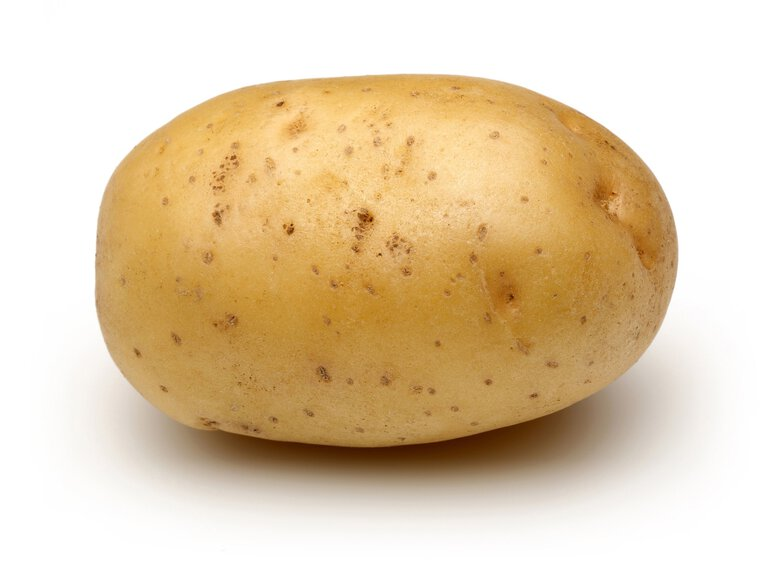
\includegraphics[width=\linewidth]{figures/potato.jpg}
  \caption{Tracks on layer 2, reference layers 1 and 3.}
  \label{fig:res_dist_L2_F13}
\end{subfigure}%
\begin{subfigure}{.5\textwidth}
  \centering
  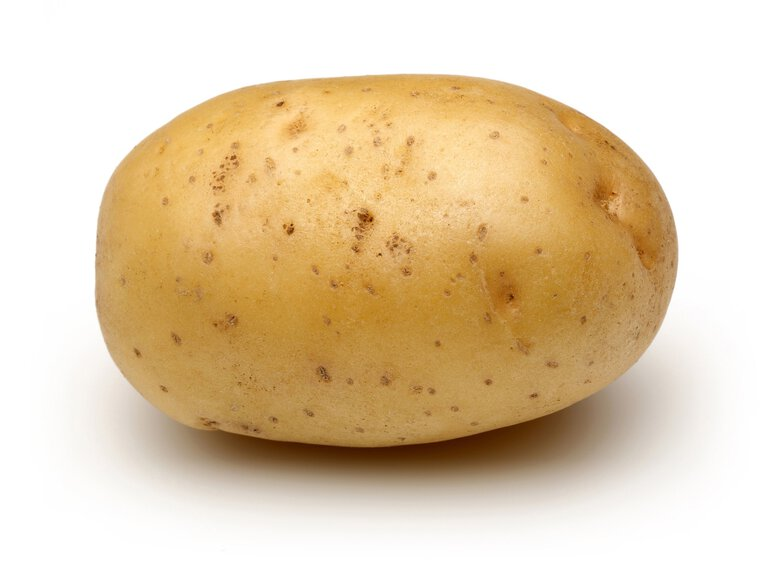
\includegraphics[width=\linewidth]{figures/potato.jpg}
  \caption{Tracks on layer 4, reference layers 1 and 2.}
  \label{fig:res_dist_L4_F12}
\end{subfigure}
\caption{Residual distribution in the region $x\in\left[xlow, xhigh\right],  y\in\left[ylow, yhigh\right] mm$ (100 mm by 100 mm area) for two different tracking combinations. }
\label{fig:res_dist}
\end{figure}

A feature of this analysis is that the residual distribution is wider for tracking combinations where the extrapolation lever arm is largest. In general, this means that residual means calculated geometrically less favourable tracking combinations have larger statistical and systematic uncertainties. The bin size of \SI{200}{\micro\meter} for the distributions shown in figure~\ref{fig:res_dist} was chosen based on the uncertainty on residuals calculated from tracks on layer 4 (1) built from hits on layers 1 and 2 (3 and 4) given a cluster y-position uncertainty of \SI{60}{\micro\meter}, since these tracks yield residuals with the largest uncertainties.

A gaussian fit was used to extract the mean of the residual distributions. Theoretically, a double gaussian distribution is more apt, but for this analysis the gaussian fit was sufficient, as discussed in appendix~\ref{appendix:systematics_res_fit_fcn}.

The motivation for the area of the region of interest will be discussed in CHAPTER 5, COMPARISON (ADD IN REF ONCE CREATED).

% --------------------------------------------------
\section{Visualizing relative misalignments between quadruplet layers}
% --------------------------------------------------

The mean of residuals was extracted for regions across entire quadruplet layers for every tracking combination to get a picture of the relative misalignments between layers. An example for QXX.X.X is shown in figure~\ref{fig:res_mean_th2}.

\begin{figure}
    \centering
    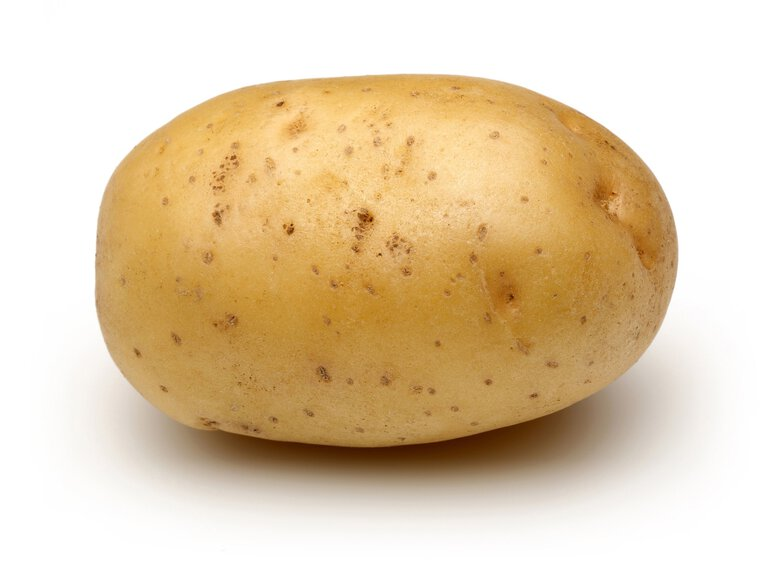
\includegraphics[width = 0.6\textwidth]{figures/potato.jpg}
    \caption{The mean of residuals represented by colour for each 100 mm by 100 mm region across layer C of quadruplet QXX.X.X for tracks built from hits on layers A and B.}
    \label{fig:res_mean_th2}
\end{figure}

\textit{on what you can see in this figure. Suggested interpretation? Potential rotation? Patterns of where there are stripes?}

Often patterns of horizontal and vertical stripes can be explained by considering regions of inefficiency, and hence less tracks, on both the layer displayed and the reference layers used to calculate the residuals. Vertical strips are typically caused by slightly less efficient wires; horizontal stripes are typically caused by the shadow of the wire supports on the three layers involved. For the example above, the number of entries in each bin in shown in figure~\ref{fig:num_entries_th2}.

\begin{figure}
    \centering
    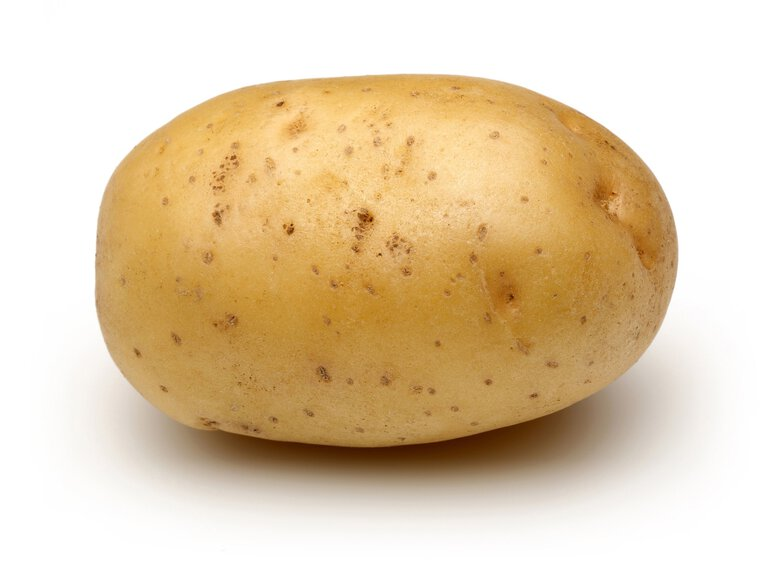
\includegraphics[width = 0.6\textwidth]{figures/potato.jpg}
    \caption{The number of residual entries in each 100 mm by 100 mm region across layer C of quadruplet QXX.X.X for tracks built from hits on layers A and B.}
    \label{fig:num_entries_th2}
\end{figure}

The local residual means will be used to validate absolute local offset measurements done by the so-called x-ray method, discussed in CHAPTER 4 X-RAY METHOD (REF ONCE CREATED).

% --------------------------------------------------
\section{Systematic uncertainty}
% --------------------------------------------------

The statistical uncertainty on the local residual means is typically around \SI{10}{} - \SI{20}{\micro\meter}, and appendix~\ref{appendix:statistics} shows that the analysis is not statistically limited by the number of triggers we collect for each quadruplet. The systematic uncertainties are more significant. 

Systematic uncertainties were assigned per tracking combination as the RMS of the distribution of the difference in local residual means calculated each with a different analysis choice. For example, the RMS associated with fitting the local residual distributions with a Gaussian or double Gaussian is \SI{25}{\micro\meter} for the geometrically least favourable tracking combinations and the distribution is shown in appendix~\ref{appendix:systematics_res_fit_fcn}.

Other choices were whether to use data collected at 2.9~kV or 3.1~kV (\ref{appendix:systematics_2900V_vs_3100V}); whether or not to apply a differential non-linearity (DNL) correction to the cluster y-positions (differential non-linearity\ref{appendix:systematics_dnl}); and what cluster fitting algorithm to use (REF ONCE YOU WRITE). A choice was made in each case, by a systematic uncertainty was assigned using the method above to account for the effect of the choice. The reasons for each choice are listed below.

Data taken at 3.1~kV was used over 2.9~kV because the strip and wire tracking efficiency increases with higher voltage.

The \package{Minuit2} package \cite{hatlo_developments_2005} was used to fit clusters over Guo's method \cite{guo_simple_2011} because it provides better and automatic statistical uncertainty estimates.

The DNL correction was not applied because its affect on the residual means was negligible.

A summary of the systematic uncertainty assigned for each choice and tracking combination is given in

%TODO : decide on an order for the table and the appendix systematics sections
%\begin{center}
\begin{tabularx}{\textwidth} {
 | >{\raggedright\arraybackslash}X 
 | >{\raggedright\arraybackslash}X 
 | >{\raggedright\arraybackslash}X
 | >{\raggedright\arraybackslash}X 
 | >{\raggedright\arraybackslash}X 
 | >{\raggedright\arraybackslash}X 
 | >{\raggedright\arraybackslash}X 
 | >{\raggedright\arraybackslash}X 
 | >{\raggedright\arraybackslash}X | }
 \hline
 \textbf{Layer} & \textbf{Fixed layer 1} & \textbf{Fixed layer 2} & \textbf{2.9~kV vs 3.1~kV} & \textbf{Residual fit function} & \textbf{Cluster fit algorithm} & \textbf{DNL} & \textbf{Total} \\ 
 \hline
 \hline
 3 & 1 & 2 & & 
 cell4 & cell5 & cell6 & 9 & 10 & 11 & 12 & 13 \\ 
 \hline
 cell7 & cell8 & cell9 & 10 & 11 & 12 & 13 & 14 \\ 
 \hline
\end{tabularx}
% \end{center}






